\section{System Architecture}
Our architecture consists of three components: mobile phones, QR codes, and a web application stack sitting in
the cloud.  The goal of our architecture is to enable virtual services on the physical world and to use the mobile
phone as an intrinsic element of those services.  An instance of our architecture was deployed inside a building and we make the
following assumptions for our archicture to deliver our goals successfully:

\begin{enumerate}
\item Most building occupants own a smartphone that they carry with them most of the time.
\item Network connectivity is available throughout the building.
\end{enumerate}
\vspace{0.06in}

Figure~\ref{fig:sysarch} shows an overview of the components of our archiecture.  We place QR codes on items throughout
the entire building.  This includes all building entrances, floors, rooms, and energy-consuming devices.  Occupants
use their phone and personal printer to add new items.  For items that are already registered, occupants use their phone
to scan their tags to learn more information about the items and to participate in maintaining a consistent
view of the building.  We discuss each of the three components in further detail in the following sections.

% Our architecture consists of various components, with the mobile phone serving as the centerpiece.  Smart phones
% serves as a point of intersection between the user, her environment, and compontational infrastructure.  Smarts phones
% are highly personalized, are carried by users everywhere, and with ubquitous, multi-modal forms of accessing a network,
% provide almost continuous access to services.  However, although space and context are nebulous ideas and difficult to capture
% we can learn from user feedback.  In order to truly bridge the physical world to the virtual world, we include the use
% of QR codes to tag \emph{any item the user finds relevant to capture}.  QR codes are easy to generate and inexpensive
% to produce and replace.

% With energy tracking as the main goal, we used QR codes to tag items that consume energy.  When an item is tagged, the user swipes
% the tag and enters information about the item.  After this `registration phase' is complete, any user can use
% their smart phone to learn about the item by swiping the QR code that is attached to it.  In addition to arbitrary
% descriptive metadata, we distinguish between regular items and \emph{meters}.  Meters are items that produce
% continuous energy data.  Meters are bound to items that are attached to them and serve as a proxy for the energy information
% about the device it is attached to.  We describe how \emph{binding} between items is done in section~\ref{sec:binding}.
% Figure~\ref{fig:sysarch} shows our system architecture and each of the components.

%FILL IN WITH REAL GRAPH
\begin{figure*}[htb!]
\begin{center}
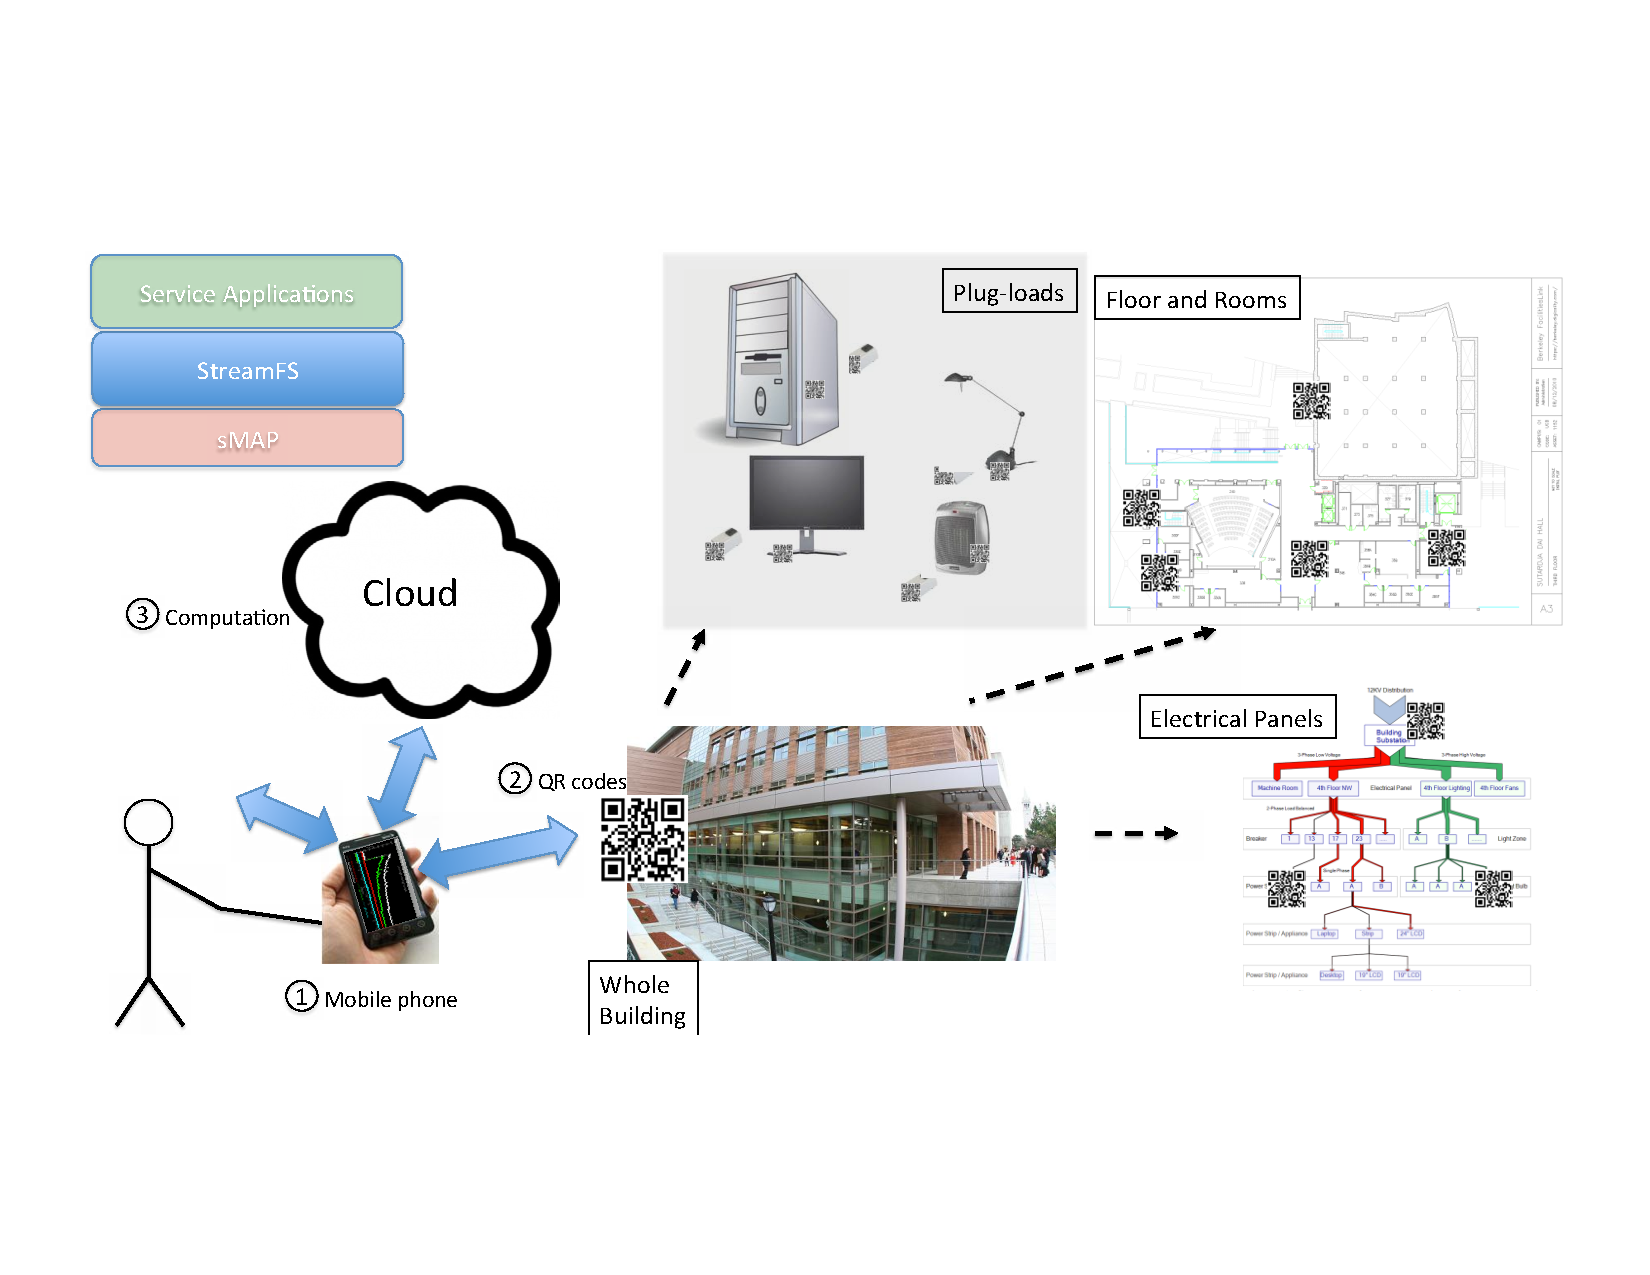
\includegraphics[width=0.8\textwidth]{figs/sysarch}
\caption{Above we show the system architecture.  The main components are mobile phone, QR codes, and access to cloud
our services.  The mobile phone serves as the triple-point of the architecture: it serves as the point of
intersection between the human, the physical world, and cloud services. }
\label{fig:sysarch}
\end{center}
\end{figure*}

\subsection{Mobile phone}
\label{sec:mobilephone}
% The mobile phone is at the center of our architecture.  Its basic function is to swipe QR codes in the environment,
% do a lookup to the backend through the network, query for any relevant information to display to the user and display it.
% Interaction with the user is through this set of displays.  For example, if a user wish to learn more about when
% their television was on, they swipe the QR code on the television.  The phone offers various services that the television
% provides.  In the current set of application we have written, you would get to read the description, make, and model of the
% television.  You might also learn what the rated power of the television, if that was included in the metadata capture.
% If the television has a meter attached and that meter is virtually and physically bound to it, on of our applications
% also allows you to view the power traces associated with television over various time intervals.  The default is 24-hours.

The mobile phone is the main component of our architecture.  It is a unique triple-point: the point of intersection
between people, physical objects, and computational infrastructure.  We take advantage of the engineering that has gone 
into making the interaction between the phone and its owner quite natural in order to give us personal and contextual
information.  For example, users naturally point towards items they are interested in capturing (when a picture is taken).
We use this gesture to capture physical objects and incorporate them in our virtual representation of the world.
People use their mobile phone camera to scan QR codes in the environment.  This can be used to obtain information
about where they are, to obtain information about the object, or to obtain information about the relationship
between objects. A simple gesture can provide the individual with a 'user
inerface' for the room and the devices within it.
\cite{Enabling ``Smart Spaces:'' Entity Description and User Interface Generation for a Heterogeneous Component-based Distributed System 
T. D. Hodes, R. H. Katz, DARPA/NIST Smart Spaces Workshop, 
Gaithersburg, Maryland, July 1998. 
UC Berkeley Technical Report CSD/98/1008}
The screen can be used as a secondary input/output to give us/them more information about the 
object or context.  We discuss these in more details in Section~\ref{sec:apps}.

\subsection{QR Codes}
\label{sec:qrc}

A QR code is a two-dimensional barcode that may encode almost 3000 bytes of data.  QR code generators
can be found on the internet~\cite{qrcgen1, qrcgen2}.  
Extending the approach in \cite{hbci}, in
our
architecture the QR code contains a meaningful {\tt URL} that a
generic browser can access to provid ea human readable document with complete
information about the item or space, as well as the additional
information to bootstrap the smartphone to optimized access, such as
native apps for interacting with the item or space.  Secondly, the 
{\tt URL}  must be easily transformed into one that will yield a
programmatic document, such as a JSON object, that apps can
manipulate.  And finally, the representation of the URL itself can be
parsed and utilized locally by native apps, typically by lookup, to
permit rapid interaction with the item or space.

\begin{figure}[htb!]
\begin{center}
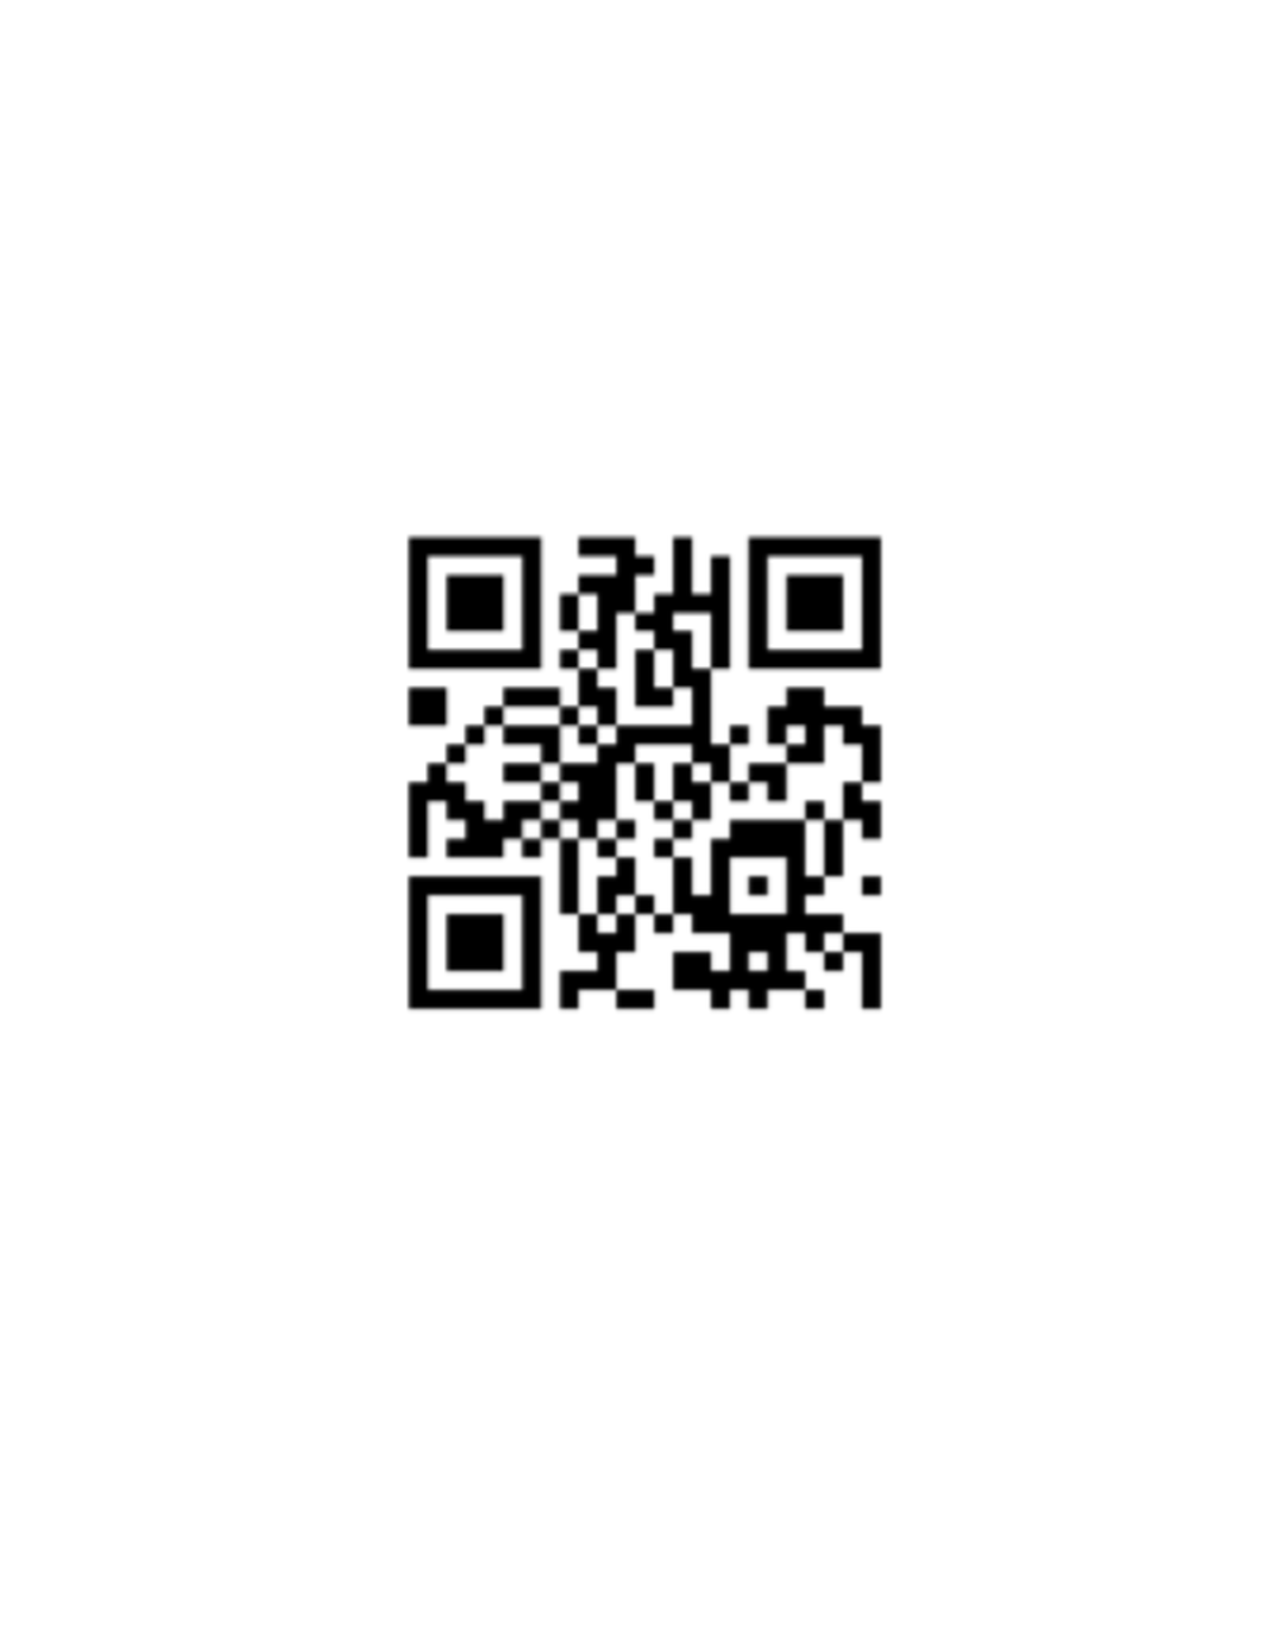
\includegraphics[scale=0.3]{figs/qrcex}
\caption{This is an example QR code from our deployment. This label resolves to {\tt http://tinyurl.com/6235eyw}.
QR codes like these are used as tags physical objects and spaces/locations.}
\label{fig:qrcex}
\end{center}
\end{figure}

Figure~\ref{fig:qrcex} shows an example QR code used in our deployment.  Tags like these are placed on physical
objects and spaces throughout the building to link between the physical world and our virtual representation of it.
QR codes are cheap to produce.  Any printer and some tape can be used to tag an item.  This is important for scalability.
With the number of physical objects and places (floors, rooms) in a typical building, {\bf we must rely on the occupants
to scale our deployment}. Because QR codes are easy to produce, we can provide occupants with a webpage that
that produces them.  They print them out, place them on items or
places they want to interact with, register them, and provide useful
information about them.

Generating the right kind of QR code is important.  It is trivial to
encode information onto them, but it is
not trivial to design them so that they encode just enough information to be useful.  If 
too much information is encode the camera takes a long time to scan them, especially under poor lighting
conditions.  This can easily frustrate and drive away users, who are critical for scalability.
We also want to design them for the lowest common denominator in terms of camera quality.  Older
phones with cheap cameras should also be able to scan the tags quickly.  We ran some experiments to show
how complex QR codes differ from the one we design and discuss these results in Section~\ref{sec:qrcodedesign}.


\subsection{Computational infrastructure}
% The third piece of our architecture consists of a data collection and management components.  The subcomponents
% of this part of the archictecture are set up in layered fashion.  The context and data mangement layer is at the top,
% the meter-access layer is below that, and at the bottom is the metering infrastructure.  The context layer sets up
% a structured metadata organization whose semantics are interpretted by each application.  We describe the single structure
% that supports our applications.  In addition, this layer unifies the metadata and the data, allowing the application
% to access all meters data that share similar properties (i.e. placement, type, owner, etc.).  The meter data-access layer 
% unifies the various access standards into a single interface.  This allows us to add sensors and easily incorporate it
% into our context layer.  Finally, we integrated various types of meter data.  Specifically, we used several wireless
% power meters called ACmes~\cite{acme} as well as various streams from the building management system directly.

The final piece of our architecture consists of three layered
components for meter and usage data representation,
data and metadata managament, and applications.  Each layer in the stack is network accessible and hosted on a combination
of machines we own and across two cloud-service providers.  The distributed nature is a testament to the flexibility of
placement for each of the pieces.  However, the layering is imposed in our setup.  Physical data streams,
coming from wireless power meters~\cite{acme}, weather feeds from weather underground~\cite{weatherunderground}, the
local building management system are directed towards the sMAP~\cite{smap}, above these feeds then forward their data
to our context management layer, StreamFS~\cite{streamfs}, and finally, we build our applications on top of StreamFS.
We describe each of these in the following sections.

\subsubsection{Application layer}
At the application layer we use a standard Apache web server~\cite{apache}.  Two of our apps -- the item
energy scanner and the personal energy counter -- are essentially just web applications.  When the phone scans a tag, it
re-directs to the main page which shows a list of services for that item that was scanned.  It also provides an option
to the user to login in to obtain a peronalized energy view.  We discuss the details of these applications as well
as the energy auditing application, which is a native app, in Section~\ref{sec:apps}.

\subsubsection{sMAP}
\label{sec:smap}
%Disucss how the streaming meter data is forwarded to streamfs and linked to streamfs objects.
sMAP~\cite{smap} provides a uniform data access layer for sensor information.  We can take any of the various sensor protocols
and make it accessible through sMAP's HTTP, RESTful API.  In addition, sMAP servers can live on any machine that is accessible
through the web.  This is convenient for our purposes, since it makes the raw sensor data stream accessible through any network.
sMAP's data-forwarding facility is used extensively to link the sensor data with the context layer.  When a meter is being added
to the context layer, a callback is installed on the sMAP server that hosts that meter's stream.  As meter data is reported 
to the sMAP server, it is forwarded to the appropriate node {\tt URL} in StreamFS, setting up the context associated with that
meter automatically.

% \subsection{Metering layer}
% We used several types of meter data in our applications.  Specifically we integrated the whole-building building power-draw feed,
% and a number of feeds from our wireless ACme power-meter deployment.

%FILL IN WITH REAL GRAPH
\begin{figure*}[htb!]
\begin{center}
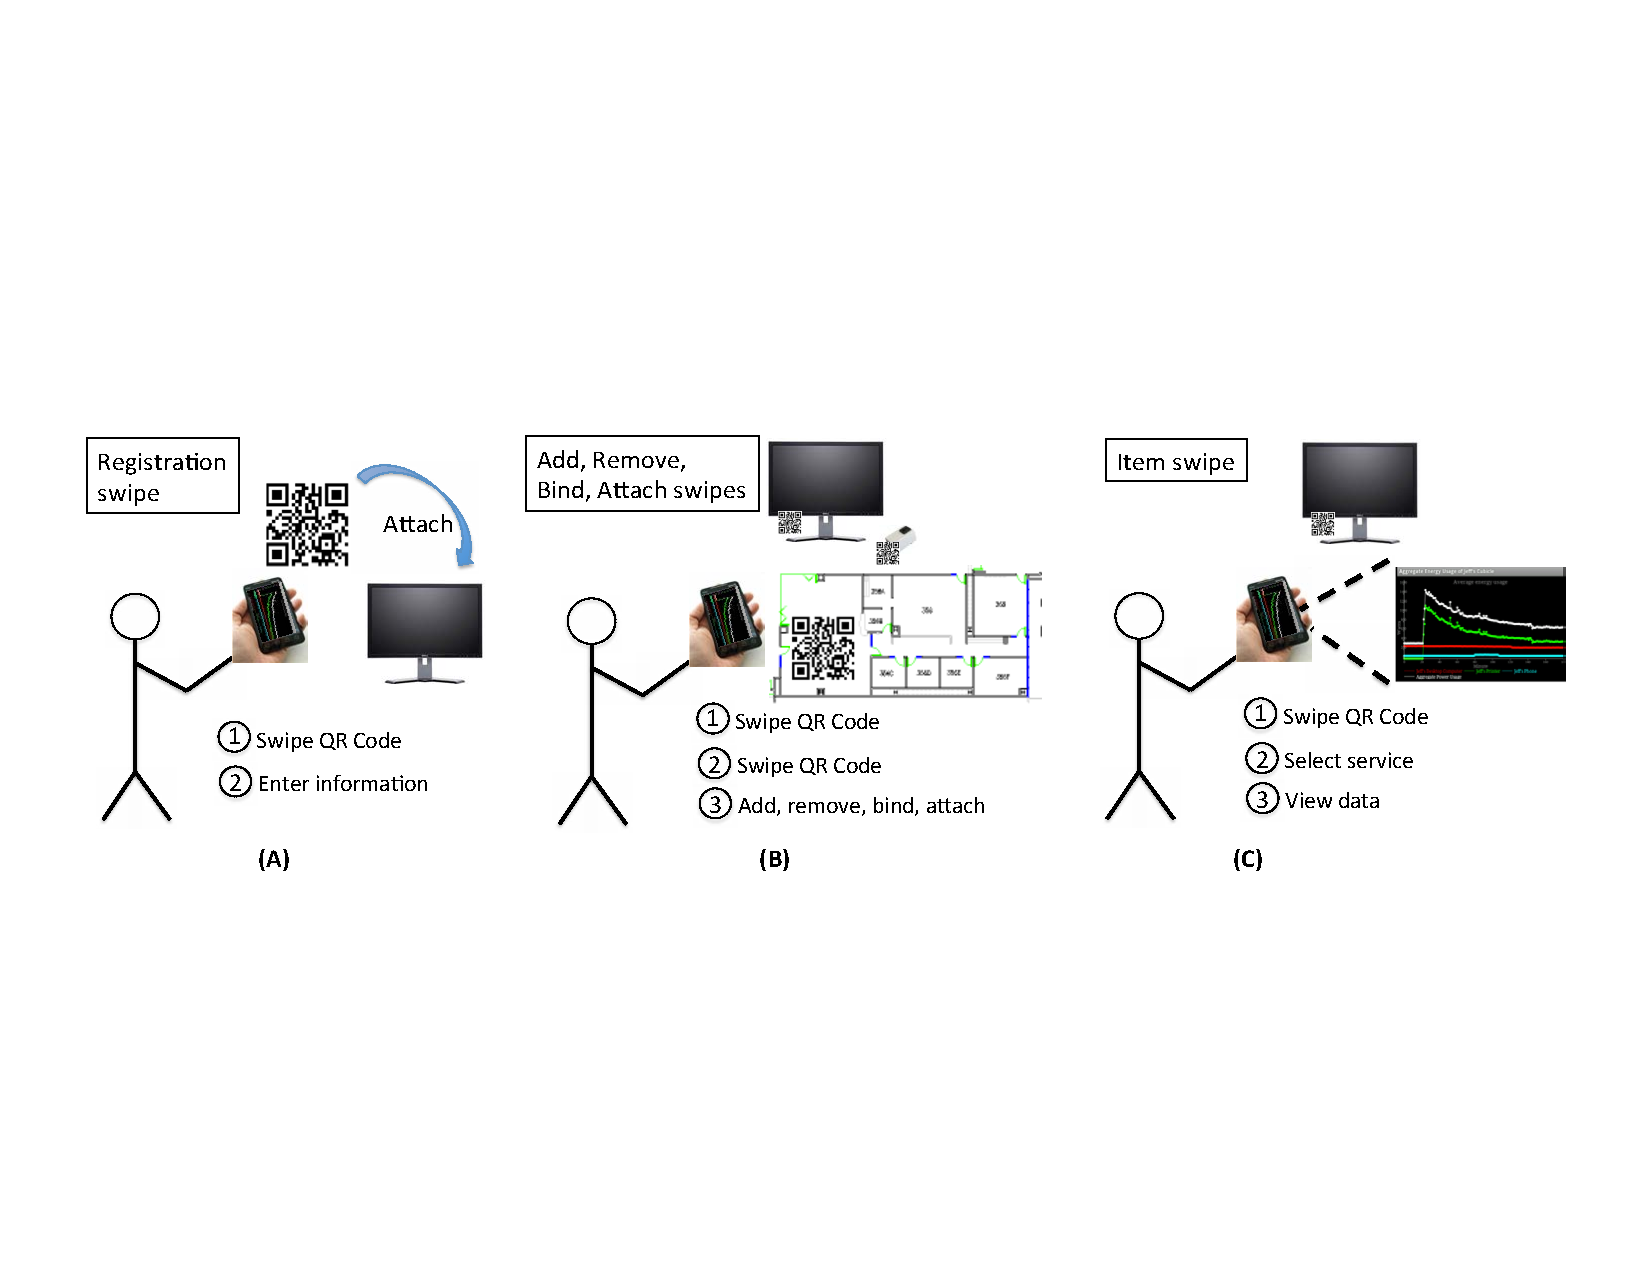
\includegraphics[width=\textwidth]{figs/swipes}
\caption{Gestures. Lorem Ipsum is simply dummy text of the printing and typesetting industry. Lorem Ipsum has 
been the industry's standard dummy text ever since the 1500s, when an unknown printer took a galley of 
type and scrambled it to make a type specimen book.  }
\label{fig:gestures}
\end{center}
\end{figure*}

\subsubsection{StreamFS}
\label{sec:streamfs}
%Discuss namespace management, binding, and recording data.
We used StreamFS~\cite{streamfs} as our data management layer.  StreamFS offers various
facilities to manage streaming sensor data and the associated metadata in a way that was useful for our the needs
of our application.  It organizes the metadata hierarchically and provides analytical
facilities that are baked into it, making it easier to create energy-analytics applications.  In particular,
StreamFS deals well with data aggregation where the number of constituents used to calculate the aggregate
changes over time.  In StreamFS, this is called \emph{dynamic aggregation} and it is described in more detail
in Section~\ref{sec:dynagg}.

Because we are fundmentally dealing with organizing data about the real-world, StreamFS is particularly useful over
a relational database abstraction.  StreamFS essentially constructs an entity-relationship graph~\cite{Chen76theentity-relationship}
and exposes this graph through a object pathnames and symbolic links.  It has been argued that semantic information
is lost in a relational data model~\cite{semanticmodel,semanticrelational}.  Our applications are built on
entity-relationship semantics, making StreamFS an ideal choice.

Each object in physical space is represented by a node in StreamFS.  Through StreamFS' RESTful/HTTP interface, we can
fetch the any node through a path rooted at the location where StreamFS is hosted.  For example, if we wish
to access the power meter in room 400 of building bldgXYZ, we may access it by issuing an HTTP {\tt GET} request to
{\tt http://server.streamfs.com/bldgXYZ/rm400/pow}.  The request returns a {\tt JSON} object with attribute-value
pairs that give a description of the temperature sensor.  It also returned that last received value from that sensor.
StreamFS provides a query interface to fetch the timeseries data collected from the sensor as well.

In addition, StreamFS support symbolic linking and this allows us to refer to nodes by multiple names.  That same 
power meter can also be referred to through {\tt /jortiz/meters/pow}; the meters that belong to user \emph{jortiz}.
More generally, StreamFS offers features that simplify namespace and data management.  Semantically, the hierarchical
node structure can be interpretted by the application.  We describe the structure and interpretation in
each application is section~\ref{sec:apps}.


\section{Gestures and QR code design}
This section briefly describes the basic primitives and design decisions that are used across all our applications.
The first is the set of gestures people perform with the smartphones to provide and obtain information about
the physical world.  The other describes our QR code design choices and why they are critical for engagement
and scalability.

\subsection{Gestures}
Mobile phones are very well engineered for incorporating natural gestures to acquire and view information.
We tried to take advantage of this by using simple gestures to obtain information about objects, context, and
movement.
Figure~\ref{fig:gestures} show the basic gestures to perform various actions.  The basic gestures fall into three
categories: registration, linking, and acquisition.  Registration is shown in the Figure~\ref{fig:gestures}(A).
It consist of a single tag swipe and entering information through the screen.  Linking gestures, 
shown is Figure~\ref{fig:gestures}(B), consist of
two swipes and the press of button to confirm the un/linking.  Finally, the acquisition swipe, shown
in Figure~\ref{fig:gestures}(C),  is a single swipe, select the data aggregate you wish to view, and viewing the data.

Each of these are natural for the user for capturing the physical world.  Swipes \emph{of}
the physical world are taken to tell us about something \emph{in} the physical world.  This makes the connection
clear to the user about the kind of information they are informing the system about.  In section~\ref{sec:apps}
we will show how gestures also tell us a just enough information to infer information about context and movement.
These gestures form the set of interaction primitives for all our
applications.  

The application logic associated with the gesture
defines the form of the relationship or action that is associated with the
gesture, such as {\tt is-in}, {\tt is-measured-by}, or {\tt
  get-control-of}.  This is in stark contrast to the use of gesture
recognition to infer actions that the person wants to perform on a
smart space.  The person takes a natural action, much like flipping on
a light switch, in order to perform an action or obtain information.
The scope of such actions is unconstrained because they are
interpreted by applications using the phone as a lens.

% \begin{itemize}
% \item Hierarchical organization
% 	\begin{itemize}
% 	\item building
% 		\begin{itemize}
% 		\item spaces
% 		\item inventory
% 		\end{itemize}
% 	\item symbolic links between spaces and inventory
% 	\item categorical
% 	\item users
% 	\end{itemize}
% \item Setting virtual view -- construction of the world
% 	\begin{itemize}
% 	\item Add/Remove through scan and input
% 	\item Un/Attaching
% 	\item Un/Binding
% 	\end{itemize}
% \item Setting context -- where in the world am i
% 	\begin{itemize}
% 	\item Check-in swipe
% 	\item Swiping items
% 	\end{itemize}
% \end{itemize}

\subsection{QR code design}
\label{sec:qrcodedesign}

An interesting observation we made in our deployments is that complex QR codes are difficult to capture and resolve
quickly, especially under poor lighting conditions.
The more data you encode on the QR code, the more 
intricate the pattern that is generated, therefore we tried to minimize the size of the {\tt URL} encoded on the QR code.  
Figure~\ref{fig:qrcexcomp} shows the difference between encoding a 
long %~\footnote{{\tt http://is4server.com/mobile/nokia/mobile.php?qrc=4eb46a8709e57}}
{\tt URL} to a short {\tt URL} shows an % http://tinyurl.com/6235eyw}.  Figure~\ref{fig:qrcexsecond} shows an 
example QR code that we used to tag items in one of our deployments.  Notice the difference between Figures~\ref{fig:qrcexfirst} 
and \ref{fig:qrcexsecond}.  The first QR code encodes 62 characters versus 26 characters for the second one.

% \begin{figure}[htb!]
% \begin{center}
% 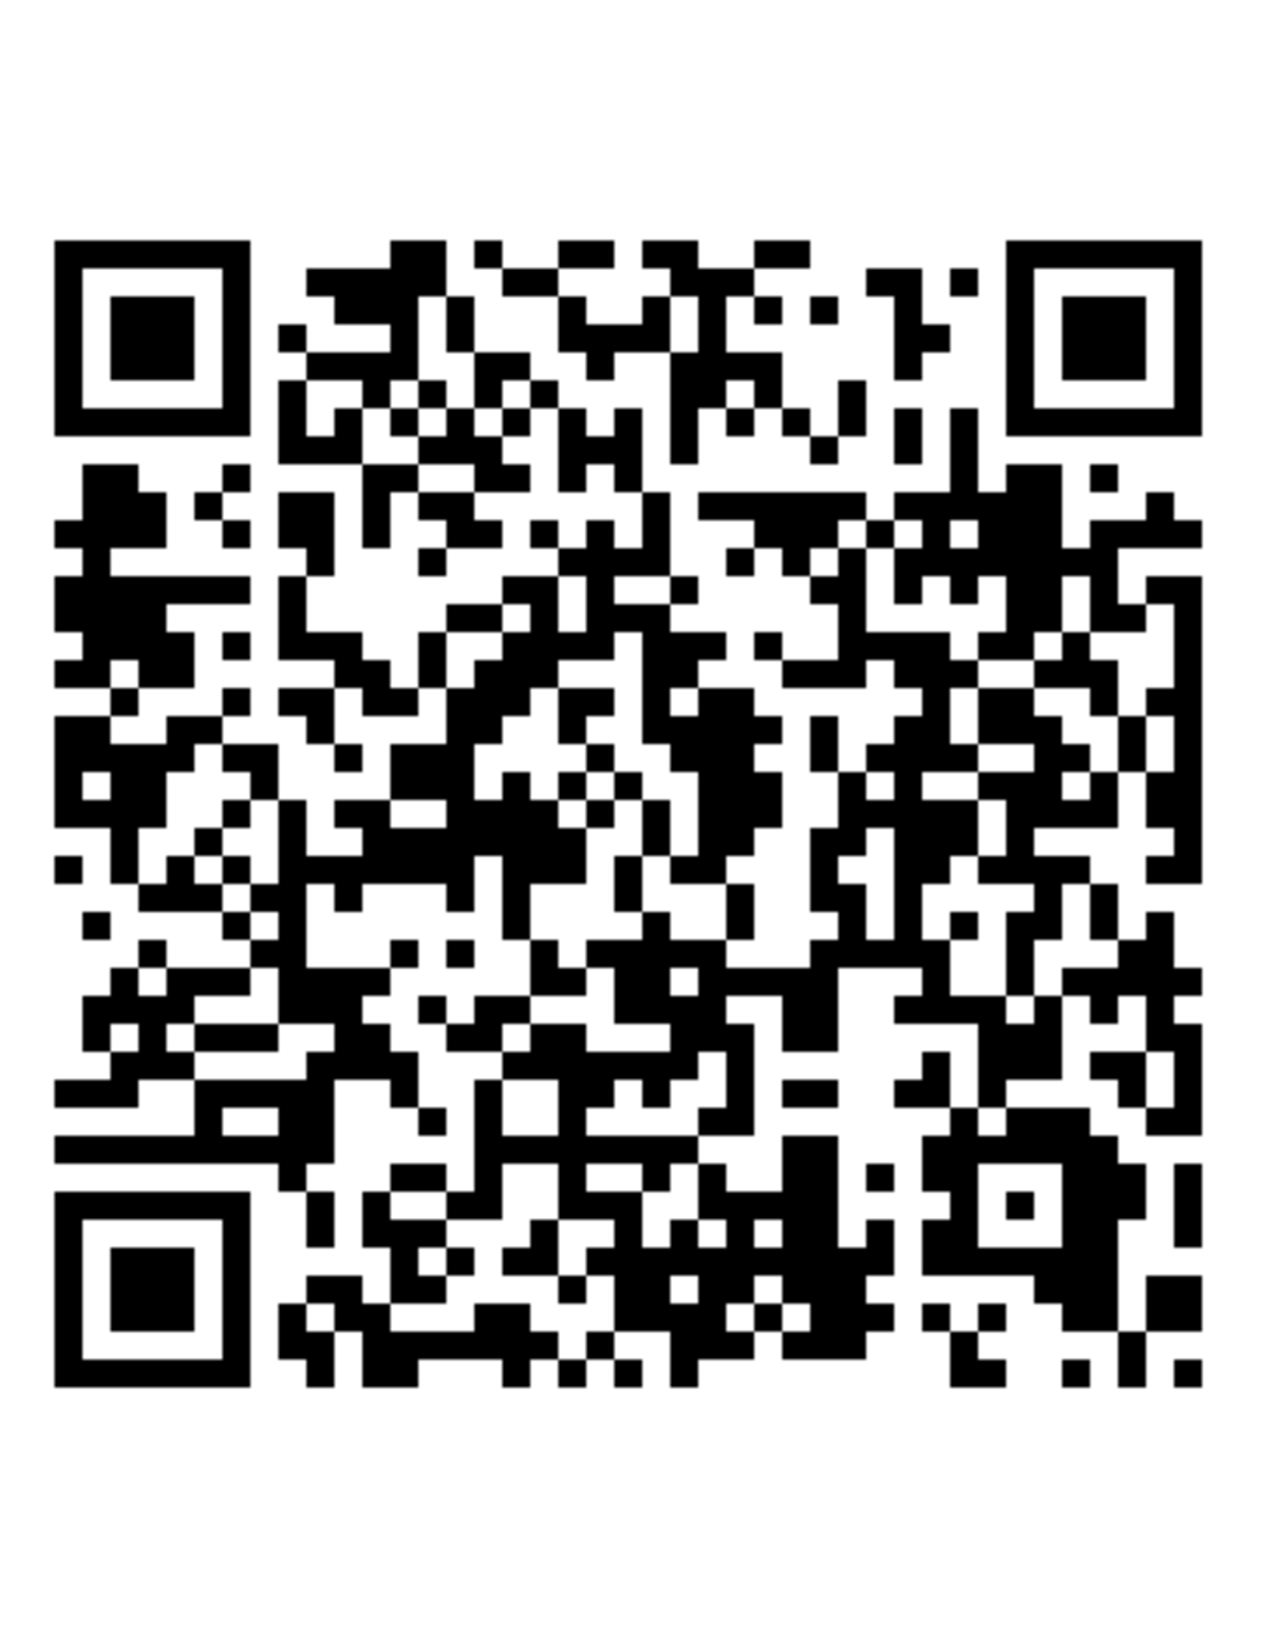
\includegraphics[scale=0.125]{figs/qrcexlong}
% \caption{This is an example QR code from our application. This label resolves to {\tt http://tinyurl.com/6235eyw}.
% We used tinyUrl to reduce the QR code image complexity and scan time.}
% \label{fig:qrcex}
% \end{center}
% \end{figure}

\begin{figure}[htb!]
\begin{center}
\subfigure[Long QR Code.]{%
            \label{fig:qrcexfirst}
            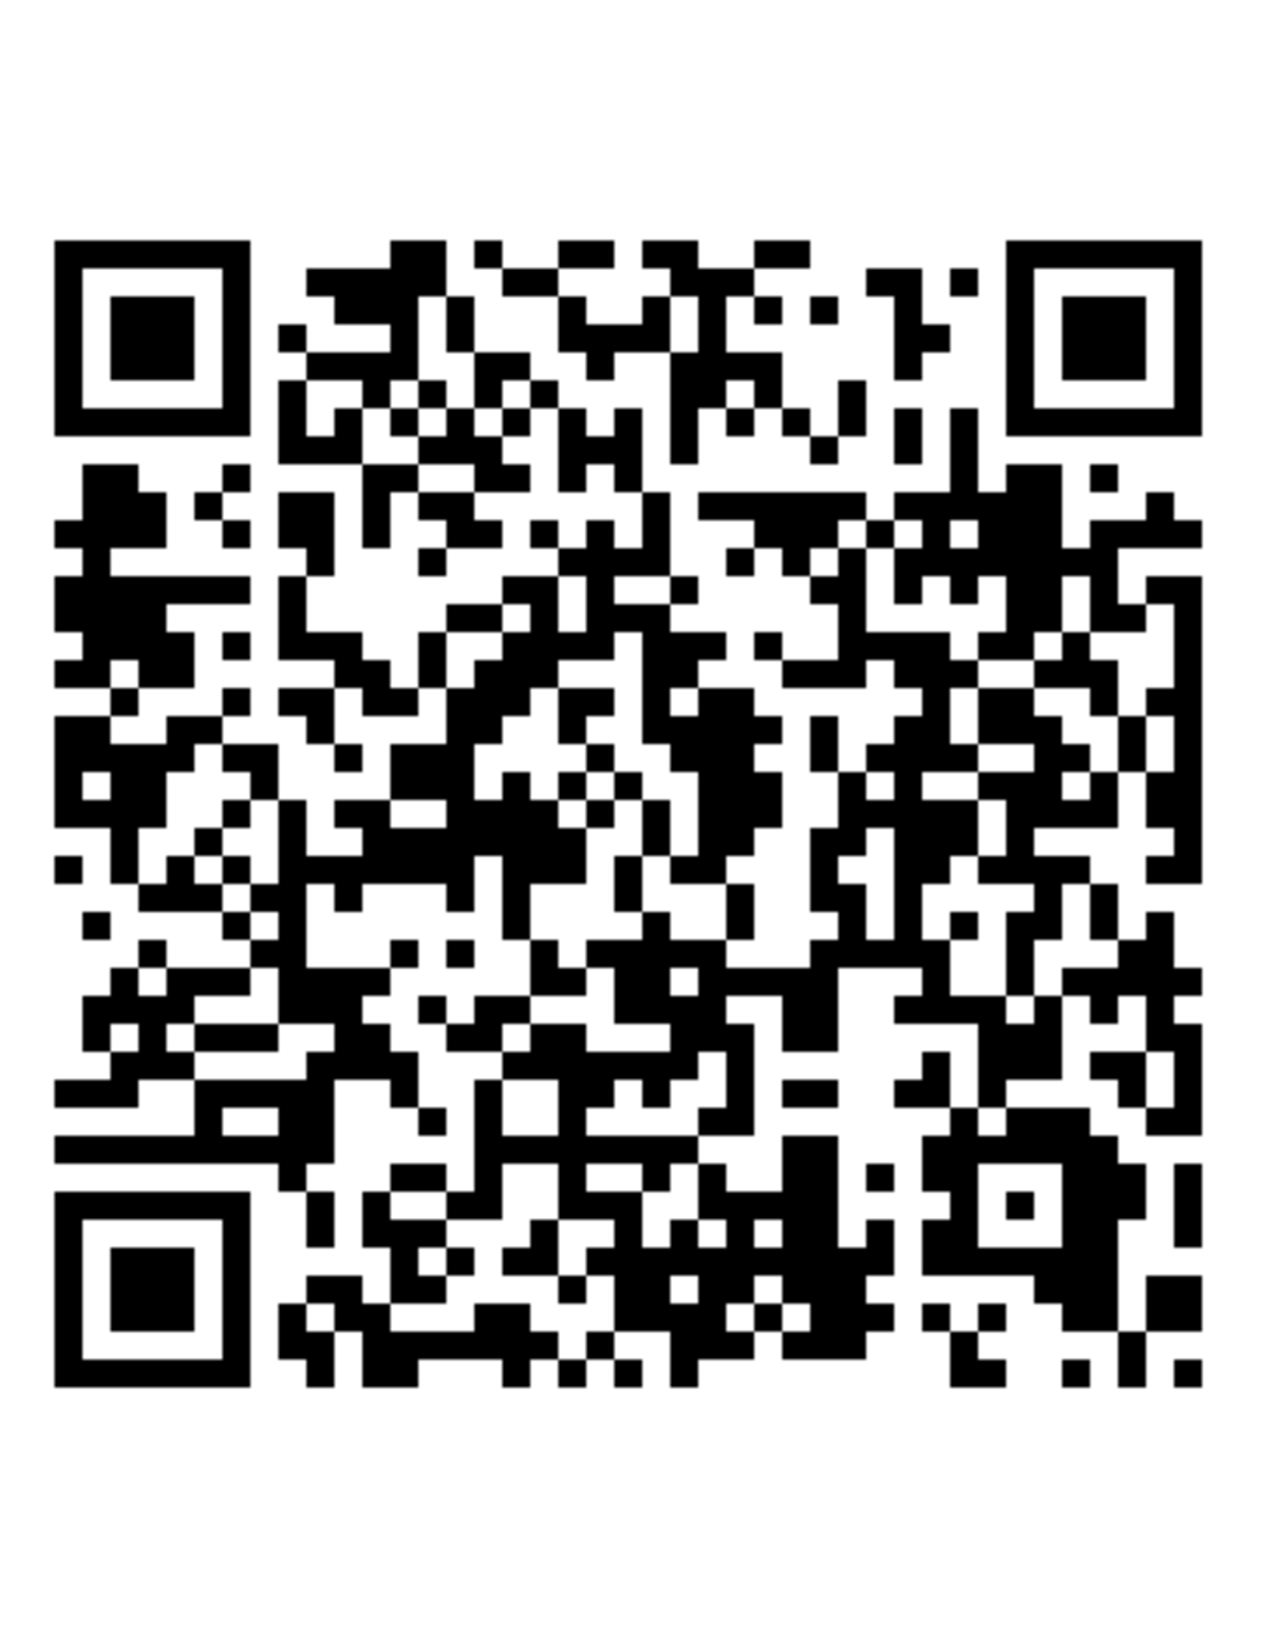
\includegraphics[scale=0.148]{figs/qrcexlong}
        }
\subfigure[Minimized QR Code.]{%
            \label{fig:qrcexsecond}
            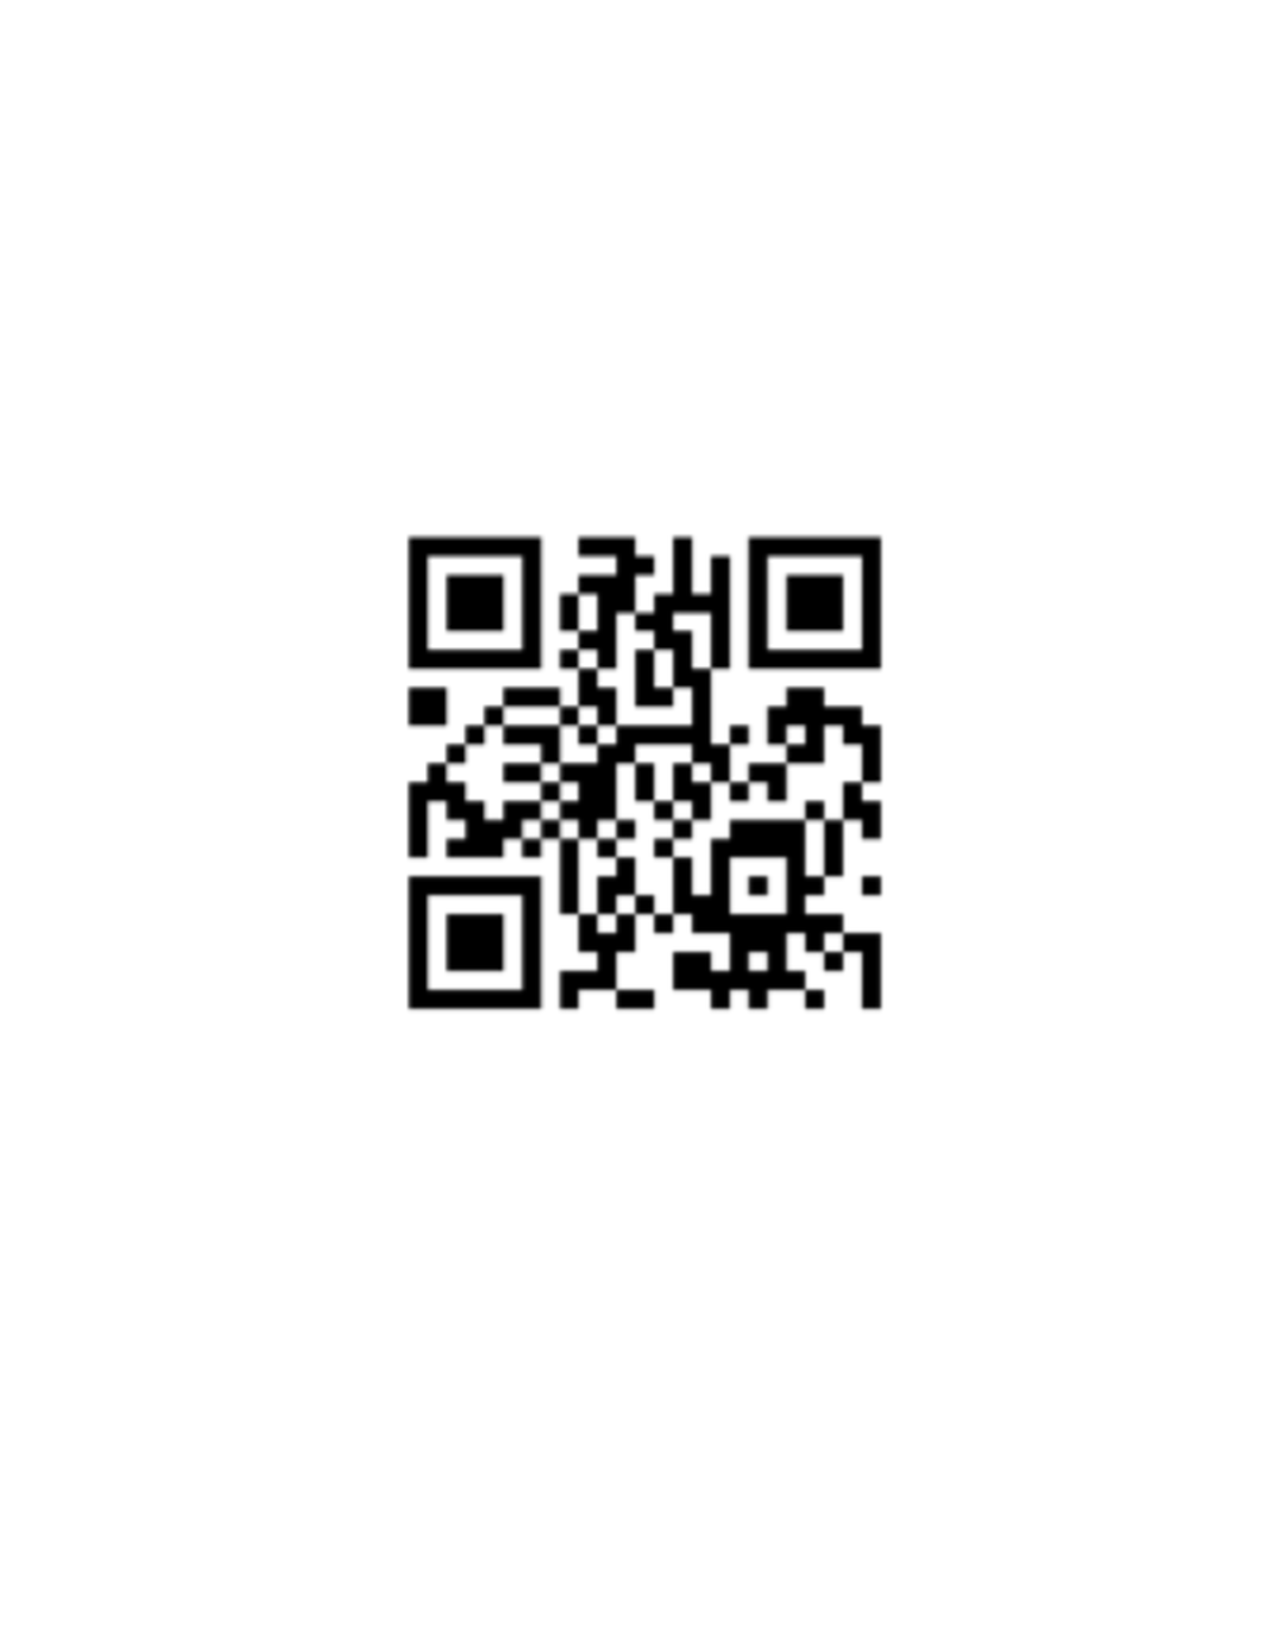
\includegraphics[scale=0.35]{figs/qrcex}
        }
\end{center}
\caption{
	The QR code on the left resolves to the same {\tt URL} at the right one, after resolution and
	redirection is complete. 
	The short label resolves to {\tt http://tinyurl.com/6235eyw}.  The second encodes about half
	the characters as the first.
	We used tinyUrl to reduce the QR code image complexity and scan time.
     }%
\label{fig:qrcexcomp}
\end{figure}

\begin{table}
\label{tab:qrscans}
\begin{center}
  \begin{tabular}{| r | c  c | }
    \hline
    			 & {\bf Average (sec) } & {\bf Variance (sec)} \\ \hline
    Short,light & 1.66 & 0.33 \\ \hline
    Short, dark & 2.08 & 0.35 \\ \hline
    Long, light & 2.26 & 0.71 \\ \hline
    Long, dark & 2.82 & 0.50 \\
    \hline
  \end{tabular}
\caption{Shows the time to scan a long QR code versus a short QR code in light and dark conditions (loosely defined).
Notice that short QR codes scan faster and with less variance that long ones.}
\end{center}

\end{table}

Table~\ref{tab:qrscans} shows the results of some simple scanning experiment between the two tags
shown above.  We scanned each QR code under light and dark lighting conditions, off the screen of my laptop.
Each experiment was run 10 times and the table shows the statistical
overview of the results. 
Clearly, scanning the simple QR code under well-lit conditions
performed the best.  The complex QR code under the same condition takes about 28-36\% longer to scan.
On a generic QR code scanner, as used here, there is a portion of the
scan time that is independent of the code complexity.  As these are
more heavily used, this is expected to be reduced substantially and
the difference is acquisition complexity will be even more pronounced.
Perhaps even more important is the variance.  Notice that the variance with the simple QR code is much smaller and
more stable under either condition.  In our experience, {\bf large variance in scan time is a major
problem for complex QR codes}.  Thus we decided to re-design our codes and push more information in the lookup
processes, as network access was more reliable than the focus of the camera on various mobile devices.
Tags are placed on all types of devices in all kinds of locations with varying degrees of lighting.
Simple QR codes are vital for widespread use.

The design choice forced us to examine others that were related.  Not being able to encode much information on 
our QR codes means we are more reliant on the network to provide the bulk of the information, to be very reliable,
and to be widespread enough that disconnection is not problematic.  Moreover, there are a number of clients
that can be used to access and display the information and the tag has to be meaningful for both.
In order to meet these criteria we (1) shrunk {\tt URL}'s using tinyURL~\cite{tinyurl} as a level of 
indirection and 
(2) designed two classes of applications: \emph{shallow} applications, and \emph{deep-inspection} applications.  Shallow
applications interact with the web-application directly while deep-inspection application use
the {\tt URL} of the web application to extract a unique identifier and provide deeper inspection
and update capabilities of the entity-relationship graph.

An example {\tt URL} we used in our deployment is {\tt http://tinyurl.com/6235eyw}.
When this is resolved, we get an empty response in the body, but we use the header to identify the QR code identifier 
that we associate with the item.  The response header looks as follows:
\begin{figure}[htb!]
\begin{center}
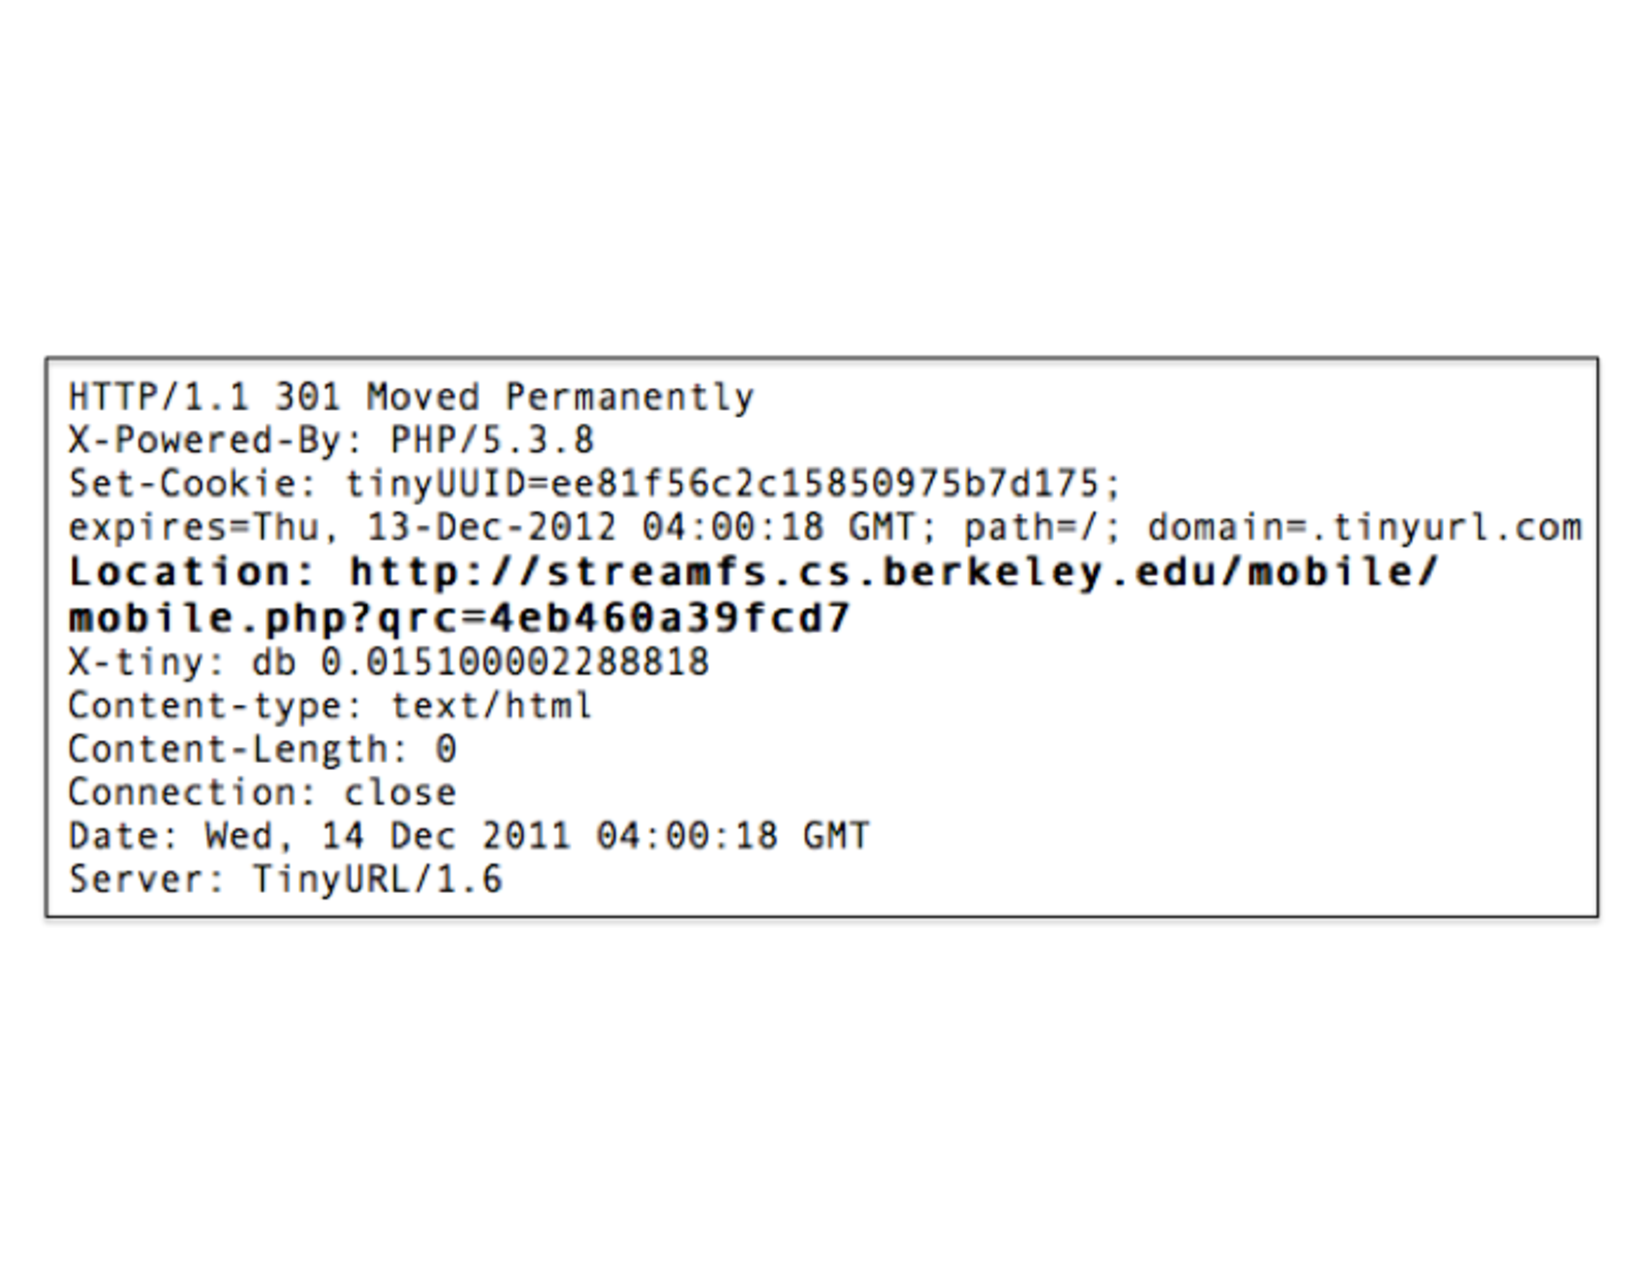
\includegraphics[scale=0.30]{figs/tinyurlhdr}
\caption{The header of the response from the {\tt tinyUrl} when resolving a QR code.  The `Location' attribute
is used to extract the unique identifier for the object this QR code tags.  It is also used to re-direct
users without the phone application to a meaningful web address for the object.}
\label{fig:tinyurlhdr}
\end{center}
\end{figure}

% It provides a web address for users to re-direct to and find information and various read-only services for the object.  However, because
% the {\tt URL} also contains a unqiue identifer \emph{qrc}, it can be used to provide for sophisticated services and capabilities.
% An example is the ability to change the virtual structure of inter-relationship between this object and other objects.  This
% is demonstrated in our energy auditing application discussed in detail in section~\ref{sec:eaudit}.
% Once items are tagged, they can be added and removed by swiping the tag and pressing the button for what you want to do with
% the item.  You also check into locations either explicit with a location-tag swipe or implicitly with an item swipe.

Notice the `Location' attribute in the header.  This is the location of the re-direct.  \emph{Shallow} applications
use the {\tt URL} directly.  The \emph{qrc} {\tt URL} is unqiue identifier for the item that this tag is attached to.
A shallow application can obtain mostly read-only service through our web applications.  For example, we'll see how
to get either item-specific data or item-aggregated data with respect to the user making the request (i.e. the total
energy consumed by \emph{my} devices).  \emph{Deep-inspection} applications are native to the phone, so we can do much
more with the tag.  Our energy auditing application allows you to related the item to other items by maintaining state of swipe
history.  This is more difficult with the web-applicaiton.  We can also use the tag and item information to couple it with
sensor information coming from sensors on the phone itself.  For example, we could determine the direction an object
is pointing by using the phone's directional sensor and negating their direction (i.e. phone is facing east, tag on item must
be facing west).







